% This document is the template for the talks given at the Matheon Center Days 30. M�rz bis 1. April 2009.
%
%Please time your presentation for 10 minutes plus 5 minutes questioning.
%
% The beamerMatheon class was created for the
%
%          DFG Research Center Matheon
%          Mathematics for Key Technologies
%
% Please send corrections and suggestions to webmaster@matheon.de
%
% use the beamer class:
\documentclass[12pt]{beamer}

% use the beamerMatheon theme with english titles
\mode<presentation>{\usetheme[language=german]{Matheon}}

% used packages
\usepackage[T1]{fontenc}
\usepackage[utf8]{inputenc}
\usepackage{amsmath}
\usepackage{amssymb}
\usepackage{alltt}
\usepackage{url}
\beamertemplatenavigationsymbolsempty
\usepackage[3D]{movie15}
%\usepackage{overpic}
\usepackage{contour} \contourlength{0.2ex}
\usepackage{array}

\def\lput(#1,#2)#3{\put(#1,#2){\hbox to 0pt{\hss{#3}}}}
\def\cput(#1,#2)#3{\put(#1,#2){\hbox to 0pt{\hss{#3}\hss}}}

\def\xw{{\mathbf x}}


% ----------- title ------------------------------------------

\title{\vspace{-1cm}Halfedge!}
\subtitle{}
\author{Stefan Sechelmann}
\date
\insertLogoTU
% \footinformation{Short title of project}

% ----------- document ------------------------------------------
\begin{document}
\maketitle


%\begin{frame}
%\frametitle{\"Ubersicht}
%\tableofcontents
%\end{frame}


% ----------- frames ------------------2-------------------------

\section{Einleitung}

%  Architekten haben Ideen unabhängig von der Ausführung
\begin{frame}
\frametitle{Plan}
\begin{center}
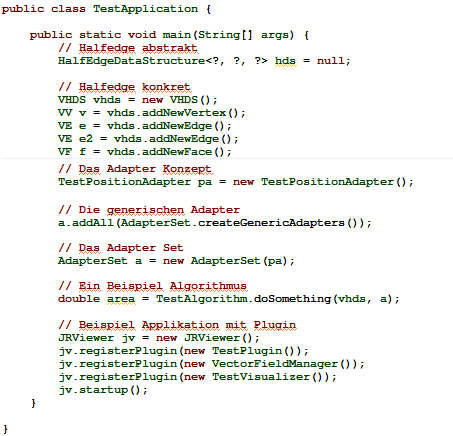
\includegraphics[height=9cm]{outline.png}\\	
\end{center}
\end{frame}

\begin{frame}
\frametitle{Halfedege konkret}
\begin{center}
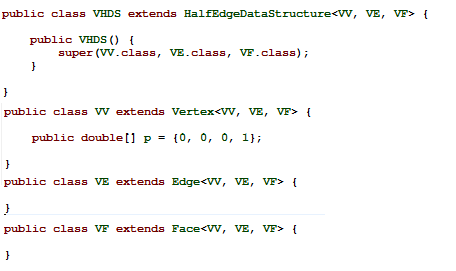
\includegraphics[height=6cm]{Vhalfedge.png}\\	
\end{center}
\end{frame}

\begin{frame}
\frametitle{Adapter Types}
\begin{center}
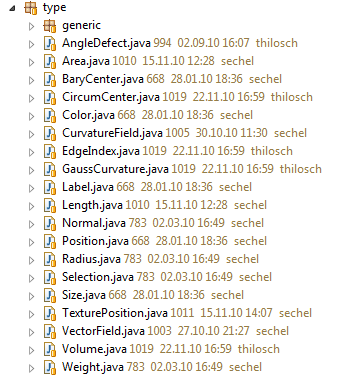
\includegraphics[height=9cm]{adaptertypes.png}\\	
\end{center}
\end{frame}

\begin{frame}
\frametitle{Generic Adapter}
\begin{center}
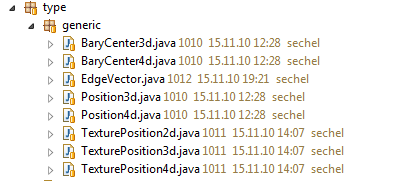
\includegraphics[height=4cm]{genericadapters.png}\\	
\end{center}
\end{frame}

\begin{frame}
\frametitle{Position Adapter}
\begin{center}
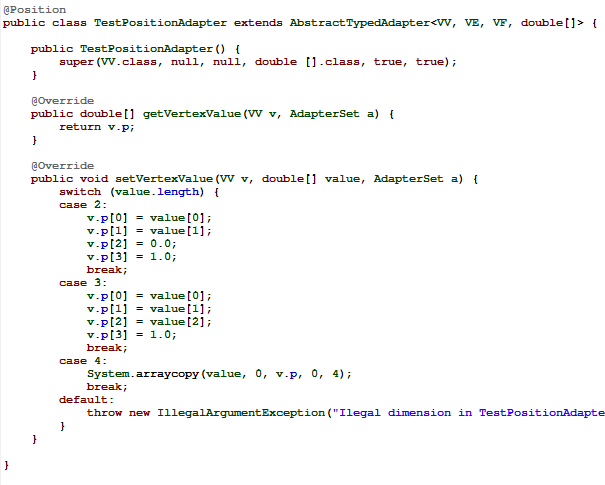
\includegraphics[height=9cm]{testadapter.png}\\	
\end{center}
\end{frame}

\begin{frame}
\frametitle{AdapterSet}
\begin{center}
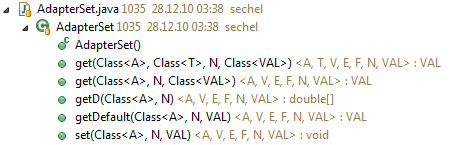
\includegraphics[height=4cm]{adapterset.png}\\	
\end{center}
\end{frame}

\begin{frame}
\frametitle{Algorithm}
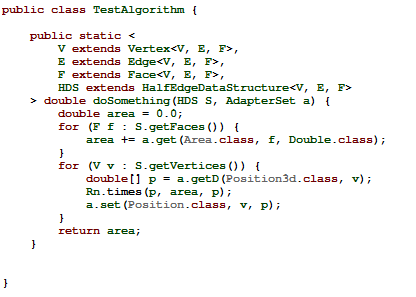
\includegraphics[height=7cm]{algorithm.png}\\	
\end{frame}

\begin{frame}
\frametitle{The Halfedge Interface}
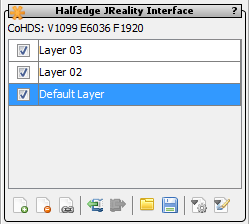
\includegraphics[height=4cm]{interface02.png}
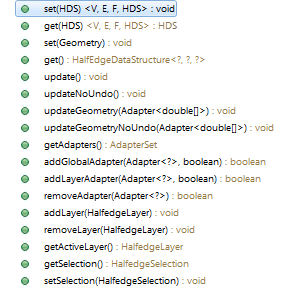
\includegraphics[height=8cm]{interface.png}
\end{frame}

\begin{frame}
\frametitle{A Halfedge Plugin}
\begin{center}
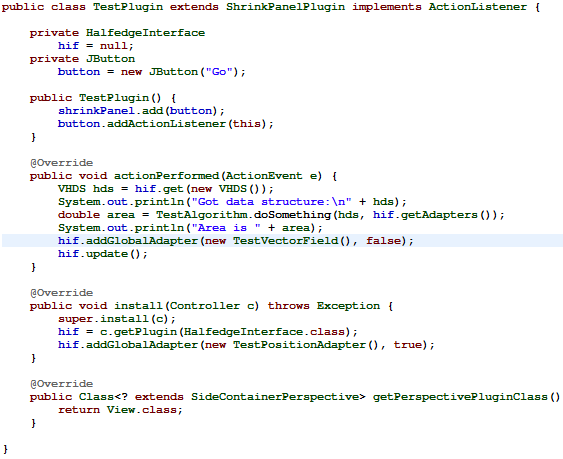
\includegraphics[height=9.8cm]{testplugin.png}\\	
\end{center}
\end{frame}

\begin{frame}
\frametitle{A Visualizer}
\begin{center}
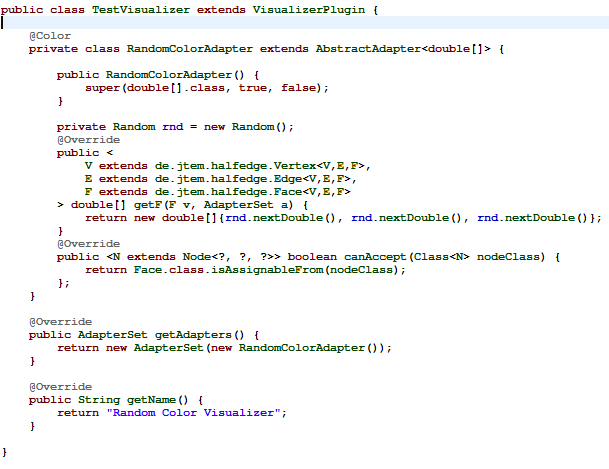
\includegraphics[height=9cm]{visualizer.png}\\	
\end{center}
\end{frame}

\begin{frame}
\frametitle{A Vector Field}
\begin{center}
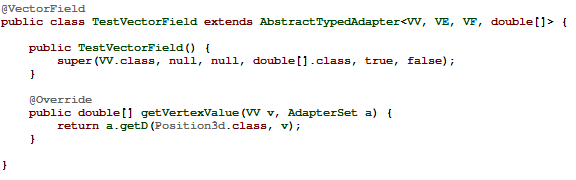
\includegraphics[height=4cm]{vectorfield.png}\\	
\end{center}
\end{frame}

\begin{frame}
\frametitle{A Scalar Function}
\begin{center}
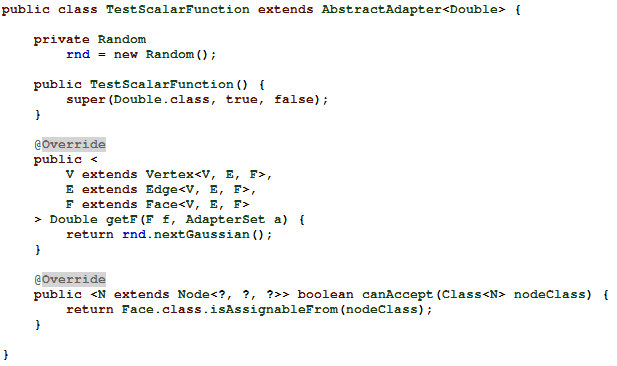
\includegraphics[height=7.4cm]{scalarfunction.png}\\	
\end{center}
\end{frame}

% \begin{frame}
% \frametitle{Pyramiden, Gizeh $2500$ v.Chr}
% \includegraphics[width=12cm]{bilder/All_Gizah_Pyramids-2.jpg}
% \end{frame}
% 
% \begin{frame}
% \frametitle{Kolosseum, Rom $80$ n.Chr}
% \includegraphics[width=12cm]{bilder/Colosseum_in_Rome,_Italy_-_April_2007.jpg}
% \end{frame}

% \begin{frame}
% \begin{center}
% \frametitle{Sears Tower, Chicago 1974}
% \includegraphics[height=9cm]{bilder/KM_6167_sears_tower_august_2007_D.jpg}
% \end{center}
% \end{frame}
% 
% \begin{frame}
% \begin{center}
% \frametitle{Grande Arche, Paris 1989}
% \includegraphics[width=11cm]{bilder/Grande-Arche.jpg}
% \end{center}
% \end{frame}
% 
% \begin{frame}
% \frametitle{The Gherkin, London 2004}
% \begin{center}
% \includegraphics[width=11cm]{bilder/London01.jpg}
% \end{center}
% \end{frame}
% 
% 
% \begin{frame}
% \frametitle{Opus, Zaha Hadid Architects, Dubai 2011}
% \includegraphics[height=7cm]{bilder/opus-rendering-02.jpg}
% \includegraphics[height=6cm]{bilder/opussubdivision01.jpg}
% \end{frame}
% 
% \begin{frame}
% \frametitle{Tanzendes Haus, Prag 1996}
% \begin{center}
% \includegraphics[height=9cm]{bilder/Prague_-_Dancing_House.jpg}
% \end{center}
% \end{frame}
% 
% 
% \begin{frame}
% \frametitle{Freiform-Architektur}
% \begin{block}{Aufgabe}
% 	Modellierung einer Glasfassade durch ungekrümmte Glasscheiben
% \end{block}
% \begin{center}
% \includegraphics[width=12cm]{bilder/opussubdivision.jpg}
% \end{center}
% \end{frame}
% 
% \begin{frame}
% \frametitle{Optimierung der Glasscheiben}
% \begin{center}
% \includemovie[
% 	mimetype=model/u3d,
% 	label=Vorher,
% 	3Djscript=Encompass.js,
% 	autoplay=true
% ]
% { 12cm }
% { 4cm }
% {models/bendflat02.u3d}
% \includemovie[
% 	mimetype=model/u3d,
% 	label=Nachher,
% 	3Djscript=Encompass.js,
% 	autoplay=true
% ]
% { 12cm }
% { 4cm }
% {models/bendflat01.u3d}
% \end{center}
% \end{frame}


\end{document}
